%!TEX TS-program = xelatex
%!TEX encoding = UTF-8 Unicode

\documentclass[12pt]{article}
\usepackage{geometry}                % See geometry.pdf to learn the layout options. There are lots.
\geometry{a4paper,top=2cm}
\usepackage[parfill]{parskip}    % Activate to begin paragraphs with an empty line rather than an indent
\usepackage{graphicx}
\usepackage{amsmath}
\usepackage{amssymb}
\usepackage{mathtools}
\usepackage{physics}
\newcommand{\be}{\begin{equation}}
\newcommand{\ee}{\end{equation}}
\usepackage[thicklines]{cancel}
\usepackage[colorlinks=true,citecolor=blue,linkcolor=blue,urlcolor=blue]{hyperref}
\usepackage{booktabs}
\usepackage{csquotes}
\usepackage{qcircuit}
\usepackage{circledsteps}
\usepackage{nicefrac}
\usepackage{fontspec,xltxtra,xunicode}
\usepackage{xcolor}
\usepackage{simplewick}
\defaultfontfeatures{Mapping=tex-text}

\newcommand{\polv}{\ensuremath{\updownarrow}}
\newcommand{\polh}{\ensuremath{\leftrightarrow}}
\newcommand{\poldr}{\rotatebox[origin=c]{45}{\ensuremath{\leftrightarrow}}}
\newcommand{\poldl}{\rotatebox[origin=c]{-45}{\ensuremath{\leftrightarrow}}}
\newcommand{\bigzero}{\mbox{\normalfont\Large\bfseries 0}}
\newcommand{\vecrp}{\ensuremath{\vec{r}^{\,\prime}}}
\newcommand{\vecnr}{\ensuremath{\vec{\nabla}_{\!r}}}

\title{Advanced Quantum Mechanics\\Class 16}
%\author{The Author}
\date{September 22, 2022}                                           % Activate to display a given date or no date

\setcounter{section}{5}
%\setcounter{subsection}{14}
%\setcounter{equation}{12}

\begin{document}
\maketitle

%%% 01

\section{Symmetries in QM}

Symmetry \(\longleftrightarrow\) conservation law.

Continuous transformations:\\
- space rotations and translations\\
- time translation

Discrete transformations\\
- space reflexion, parity\\
- charge conjugation

Space is isotropic and homogeneous, and
the description of an isolated system should not
depend on the origin of time.
An additional requirement: laws of physics do not
change in going from one inertial frame to another.

When talking about changes in reference frames,
important to distinguish two viewpoints:

\emph{Passive:}
Physical system is not
changed, but the axes
and time scales are
changed.

\emph{Active:}
Axes and clocks are not
changed, symmetry operation
is applied to the physical
system.

Example: spatial translation.

Active -- point is dislocated, \(\vec{r}\) and \(\vec{r}^{\,\prime}\) measured
with respect to the same origin
\be
\vec{r}^{\,\prime}=\vec{r}+\vec{a}
\ee

%%% 02

Passive -- axis is dislocated,
\be
\begin{array}{l}O^{\prime}=O+\vec{a} \\ 
\vec{a}+\vec{r}^{\,\prime}=\vec{r} \\ 
\boxed{
\vec{r}^{\,\prime}=\vec{r}-\vec{a}
}\end{array}	
\ee
origin dislocated to \(O^{\prime}\) with respect to \(O\),
\(\vec{r}^{\,\prime}\) is the position with respect to \(O^{\prime}\) .

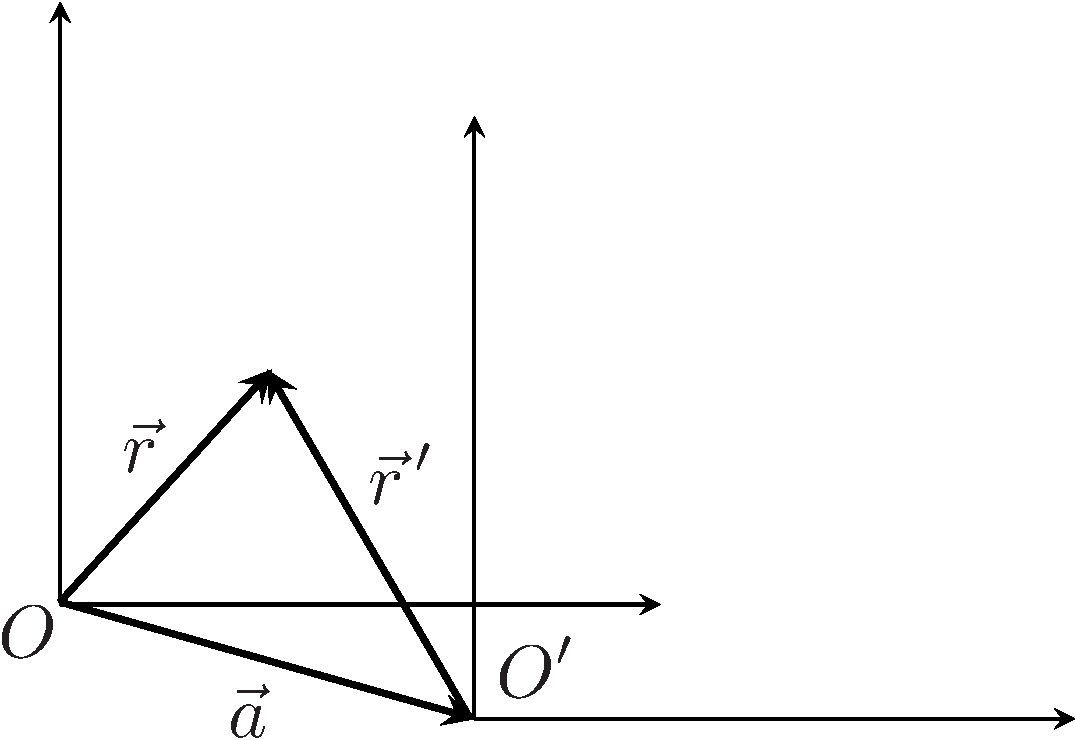
\includegraphics[width=0.45\textwidth]{Figures/PassiveTransformation-crop.pdf}\hfill%
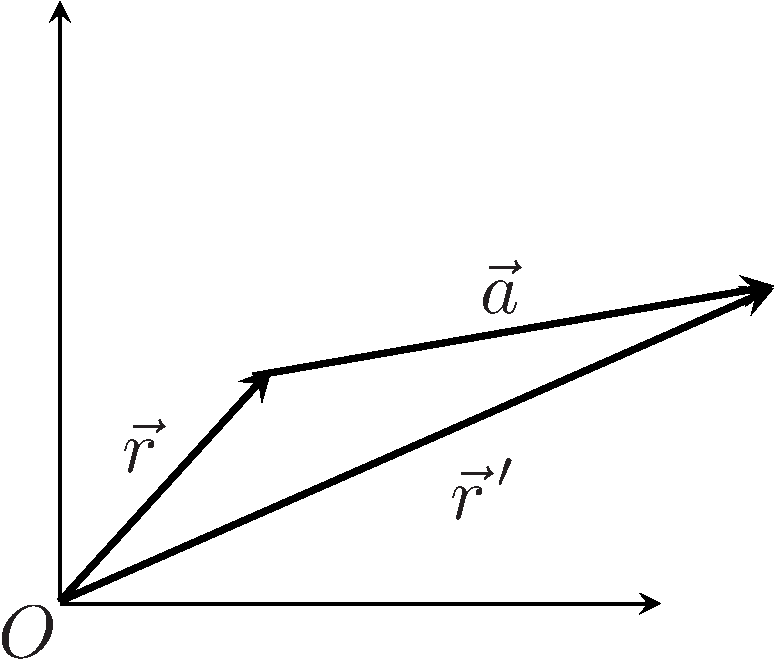
\includegraphics[width=0.35\textwidth]{Figures/ActiveTransformation-crop.pdf}\\
\begin{center}
Left: passive transformation. Right: active transformation.
\end{center}

A passive translation of \(-\vec{a}\) leads to a position
vector whose expression is identical to an active
translation defined by a vector \(+\vec{a}\).

\emph{Warning:}
mixing the two viewpoints in the
same calculation can lead to
grotesque erros $\rightarrow$
or looking up equations in
books using different viewpoints.

Here, use of the active point of view. Also, for
the following discussion, it is important to
restate Postulate I in terms of rays:
\begin{itemize}
\item Physical state is a normalized ray in the
space of states H \(\Rightarrow\) a normalized vector up
to a phase.
\end{itemize}

%%% 03 OKAY

Physical state is not represented by a single vector
in Hilbert space \(\Rightarrow\) but by an entire collection of
unit vectors. This introduces a complication when
discussing a symmetry a transformation (``does nothing
to the physical system''):
\begin{itemize}
\item under a symmetry transformation, 
one \emph{cannot} restrict it to mapping a vector in
H into some vector in H
$\rightarrow$
symmetry transformation maps a set
of vectors differing by a phase into another
set of vectors that differ by a phase; it is
a ray-into-a-ray mapping;
%
\item
but ``to do nothing to a physical system'', \textit{i.e.} to
be a symmetry, such a mapping must preserve
probabilities (absolute values (moduli) of scalar
products of state vectors).
\end{itemize}

Let \(\widetilde{\varphi}\) denote the whole set of vectors that
differ from each other by a phase:
\be
\widetilde{\varphi}=\left\{e^{i \theta}|\varphi\rangle, \theta\right. \text{real} \}
\ee
Let $g$ denote a transformation on the apparatus
%%% 04 OKAY
preparing the state \(\widetilde\varphi\), i.e.
\be
\widetilde{\varphi}_{g}: \widetilde{\varphi} \rightarrow \widetilde{\varphi}_{g}
\ee
then
$g$ transforms a collection of state vectors, \(\widetilde{\varphi}\),
in to another collection of state vectors, \(\widetilde{\varphi}_{g}\)

Then, if we perform the same transformation on
the measuring device for a state \(\widetilde{\chi}\), \textit{i.e.}
\be
\widetilde{\chi}_{g}: \widetilde{\chi} \rightarrow \widetilde{\chi}_{g}
\ee
to be a symmetry, one must have
\be
\left|(\widetilde{\chi}_{g} | \widetilde{\varphi}_{g})\right|^{2}=|(\chi | \varphi)|^{2}
\label{eq:symmetry1}
\ee
where \((\widetilde{\chi}_{g}|\widetilde{\varphi}_{g})\) 
denotes the scalar product of
one of the state vectors in the set \(\widetilde{\varphi}\) and one
of the state vectors of the set \(\widetilde{\chi}\).
\((\widetilde{\chi} | \widetilde{\varphi})\) 
\emph{does not} denote a scalar poduct
between the rays \(\widetilde{\varphi}\) and \(\widetilde{\chi}\), such a product
is meaningless.

\emph{Wigner theorem:}
there are only two ways that
Eq.~\eqref{eq:symmetry1} can be satisfied for
all vectors in \(\widetilde{\varphi}\) and \(\widetilde{\chi}\):
%%% 05 OKAY
it is possible to choose a representative state
vector \(\left|\varphi_{g}\right\rangle\) in the set \(\widetilde{\varphi}\) such that for any
state vector \(|\varphi\rangle \in H\) :
\be
\left|\varphi_{g}\right\rangle=\hat{U}(g)|\varphi\rangle
\ee
where \(U(g)\) is unitary or antiunitary, with
\(\hat{O}(z)\) being unique up to a phase.

\emph{$\hat{U}(g)$ unitary}:
\be
\left\langle \chi_{g} | \varphi_{g}\right\rangle=\langle\hat{U}(g) \chi | \hat{U}(g) \varphi\rangle=\langle \chi | \varphi\rangle
\ee
absolute value (norm) and phase
of the scalar product are preserved.

\emph{$\hat{U}(g)$ antiunitary}:
\be
\begin{aligned}
\left\langle \chi_{g} | \varphi_{g}\right\rangle 
&=\langle\hat{U}(g) \chi | \hat{U}(g) \varphi\rangle \\ 
&=\langle \chi | \varphi\rangle^{*}=\langle\varphi | \chi\rangle 
\end{aligned}
\ee
and the phase of scalar product is \emph{not} preserved.
Needed for time-reversal transformation only
-- for now, we consider unitary \(\hat{U}\) only.
This has interesting consequences when $g$ forms a group.

%%% 06 OKAY

\subsection{Groups}

Let \(g\) denote a group of transformations, and \(g_{1}, g_{2}, \ldots\)
its elements:
\begin{itemize}
\item closure:
\be
g_{1}, g_{2} \in G \Rightarrow g_{2} g_{1}=g \in G
\ee
where we mean successive applications,
first $g_1$, then $g_2$.
\[
\text { order is important }
\left\{
\begin{aligned}
g_{1} g_{2} &=g_{2} g_{1} \text { Abelian } \\ 
g_{1} g_{2} &\neq g_{2} g_{1} \text { non-Abelian }
\end{aligned}
\right.
\]
%
\item product is associative:
\be
g_{1}, g_{2}, g_{3} \in G
\Rightarrow
g_{1}(g_{2} g_{3})=(g_{1} g_{2}) g_{3}
\ee 
%
\item there exists the \emph{identity} (neutral element):
\be
g = I
\ee
which does nothing.
%
\item for each $g$, there is an inverse $g^{-1}$:
\be
g^{-1} g=gg^{-1}=I
\ee
\end{itemize}


\subsection{Vector and spinor representations}

Vector and spinor representations of $g$ in $H$.
Choice of phases of \(|\varphi\rangle\) and \(\left|\varphi_{g}\right\rangle\) such that \(\left|\varphi_{g}\right\rangle=\hat{U}(3)|\varphi\rangle\)
%
\be
g=g_{2} g_{1}
\left\{
\begin{aligned}
\left|\varphi_{g}\right\rangle
&=\hat{U}(g)|\varphi\rangle \\
\left|\varphi_{g_{2} g_{1}}\right\rangle
&=\hat{U}(g_{2})\left|\varphi_{g_{1}}\right\rangle
 =\hat{U}(g_{2}) \hat{U}(g_{1})|\varphi\rangle
\end{aligned}
\right.
\ee
\(\left|\varphi_{g}\right\rangle\) and
\(\left|\varphi_{g_{2} g_{1}}\right\rangle\) 
are identical physical states \(\rightarrow\) must be up equal to a phase.
%
\be
\left|\varphi_{g}\right\rangle=e^{i \alpha(g_{2}, g_{1})}\left|\varphi_{g_{2} g_{1}}\right\rangle
\label{eq:symmetries2}
\ee
\emph{Exercise:} $\alpha$ is independent of $\ket{\varphi}$.
%%% 07 OKAY

From Eq.~\eqref{eq:symmetries2}, since $\ket{\varphi}$ is arbitrary:
\[
\hat{U}(g)=e^{i \alpha(g_{2}, g_{1})} \hat{U}(g_{2}) \hat{U}(g_{1})
\left\{
\begin{aligned}
+\hat{U}(g_{2}) \hat{U}(g_{1}) 
&\text{ -- vector repr.}\\
\pm\hat{U}(g_{2}) \hat{U}(g_{1}) 
&\text{ -- spinor repr.}
\end{aligned}
\right.
\]

\subsection{Infinitesimal generators}

Infinitesimal generators 
for continuous transformations, represented
by an important class of groups: \emph{Lie groups}.
Example: rotation group \(S O(3)\), group of orthogonal
matrices \(R^{T} R=RR^{T} =I\), where  \(T\) is transpose,
is a \emph{3-parameter group}.
The 3 parameters can be, \textit{e.g.}
\(n\) rotation axis
2 angles in \(O_{xyz}\) + 
rotation angle about \(\hat{n}\).

Rotation group has 3 Abelian subgroups,
rotations about a fixed axis, that taken together
describe an arbitrary rotation in 3-dim space,
three independent parameters (\emph{e.g.} Euler angles).

In general, a Lie group \(G\) is parametrised by
\(n\) independent parameters: dimension of \(G\).
Consider an Abelian (sub)group with elements \(h\)
parametrised by an additive parameter \(\alpha, h=h(\alpha)\):
\be
h\left(\alpha_{1}+\alpha_{2}\right)=h\left(\alpha_{2}\right) h\left(\alpha_{1}\right)=h\left(\alpha_{1}\right) h\left(\alpha_{2}\right)
\ee

%%% 08 OKAY

Representation of $h$ in $H$: $\hat{U}_h(\alpha)$
\be
\hat{U}_h(\alpha_1+\alpha_2) = \hat{U}(\alpha_2)\hat{U}(\alpha_1) = \hat{U}(\alpha_1)\hat{U}(\alpha_2)
\ee
that, via the Stone theorem, leads to:
\be
\hat{U}(\alpha) = e^{-i\alpha \hat{T}_h}
\ee
$\hat{T}_h$: infinitesimal generator, Hermitian: associated with a physical property.

\begin{itemize}
\item Time translations:
\be
\hat{U}(t)=e^{-i / \hbar \hat{H} t} \quad,\quad \hat{T}=\hat{H}
\ee
%
\item Space translations: $\vec{a}=a \hat{a}$
\be
\hat{U}(\vec{a})=e^{-i / \hbar \vec{a} \cdot \hat{\vec{P}}} \quad,\quad \hat{T}=\hat{\vec{P}} \rightarrow \text{ momentum}
\ee
%
\item Space rotation by $\theta$ about a direction $\hat{n}$:
\be
\hat{U}_{\hat{n}}(\theta)=e^{-i / \hbar \theta \hat{J}_{\hat{n}}} \quad,\quad \hat{T}=\hat{n} \cdot \vec{J} \rightarrow \text{ ang. momentum}
\ee
%
\item Spatial boosts, Galilean transformation of the velocity $\vec{v}$:
\be
\hat{U}(\vec{v})=e^{-i / \hbar \vec{v} \cdot \vec{G}} \quad,\quad \hat{T}=\vec{G}=-m \vec{R} \rightarrow \text{ mass and position}
\ee
\end{itemize}

\subsection{Lie Algebra of a continuous group}

Let us examine the properties of a Lie group in the
vicinity of the identity \(\rightarrow\) find the algebra of the generators.

%%% 09 OKAY

\(N\) coordinates \(\theta_{a}, a=1,2, \ldots, N\), with
\be
g(\theta=0)=I
\ee

Composition law:
\be
g(\overline{\theta}) g(\theta)=g(f(\overline{\theta}, \theta))
\ee
notation:
\be
\theta=\{\theta_{a}\}, f(\overline\theta, \theta)=\{f_{a}(\theta_{b}, \theta_{c})\}
\ee
with $f$ infinitely differentiable in $\overline{\theta}_a,\theta_a$.

A representation in $H$:
\be
\hat{U}(\overline{\theta}) \hat{U}(\theta)=\hat{U}(f(\theta, \theta))
\label{eq:symmetries3}
\ee
For $\theta = 0$:
\be
\begin{aligned} 
g(\overline{\theta}) g(\theta) &=g(f(\overline{\theta}, \theta)) \\ 
\downarrow \quad\,\\ 
I \quad\,& \rightarrow f(\overline{\theta}, 0)=\overline{\theta}
\end{aligned}
\ee
%
For $\overline\theta = 0$:
\be
\begin{aligned} 
g(\overline{\theta}) g(\theta) &=g(f(\overline{\theta}, \theta)) \\ 
\downarrow \quad\quad\quad\\
I\quad\quad\quad& \rightarrow f(0, \overline{\theta})=\theta 
\end{aligned}
\ee
%
For $\overline\theta = \theta = 0$:
\be
\begin{aligned} 
g(\overline{\theta}) g(\theta) &=g(f(\overline{\theta}, \theta)) \\ 
\downarrow \quad\downarrow\quad\\
I\quad I\quad & \rightarrow f(0, 0)=0
\end{aligned}
\ee
Taylor expanding $f(\overline\theta,\theta)$ up to second order in $\theta,\overline\theta$
\be
\begin{gathered}
f_a(\overline{\theta}, \theta)=0+\overline{\theta}_{a}+\theta_{a}+\left.\frac{1}{2} \frac{\partial^{2} f_{a}}{\partial \overline{\theta}_{b} \partial \overline{\theta}_{c}}\right|_{0} \overline{\theta}_{b} \overline{\theta}_{c}\\
%%% 10 OKAY
+\left.\frac{1}{2} \frac{\partial^{2} f_{a}}{\partial \theta_{b} \partial \theta_{c}}\right|_{0} \theta_{b} \theta_{c}+
\frac{\partial^{2} f_{a}}{\partial \theta_{c} \partial \theta_{b}} \theta_{c} \theta_{b}+\cdots
\end{gathered}
\ee
with
\be
\frac{\partial^{2} f_{a}}{\partial \theta_{c} \partial \theta_{b}}  = f_{abc}
\ee
and a sum over repeated indices is implied. Since
\be
\left.
\frac{\partial^{2} f_{a}}{\partial \overline\theta_{c} \partial \overline\theta_{b}}
\right|_{\overline\theta=0,\theta=0}
=
\left.
\frac{\partial^{2}}{\partial \overline\theta_{c} \partial \overline\theta_{b}}
\underbrace{f(\overline{\theta},0)}_{\overline\theta}
\right|_{\overline\theta=0}
= 0 
\ee
and similarly for $\partial^{2} f_{a} /\left.\partial \theta_{b} \partial \theta_{c}\right|_{0}=0$. Therefore
\be
f(\overline{\theta}, \theta)=\overline{\theta}_{a}+\theta_{a}+f_{abc} \overline{\theta}_{b} \theta_{c}+\ldots
\ee

Expansion of $\hat{U}(\theta)$ up to second order in $\theta$:
\begin{align}
\hat{U}(\theta) 
&\simeq I- i \theta_{a} \hat{T}_a-1 /2 \left.\frac{\partial^{2} \hat{U}}{\partial \theta_{a} \partial \theta_{b}}\right|_{0} \theta_{a} \theta_{b}+\ldots\\
&=I-i \theta_{a} \hat{T}_{a}-1 / 2 \theta_{a} \theta_{b} \hat{T}_{a b}+\cdots
\end{align}
with
\[
\left.\frac{\partial^{2} \hat{U}}{\partial \theta_{a} \partial \theta_{b}}\right|_{0} = \hat{T}_{ab} = \hat{T}_{ba}
\]
and we use in the composition law Eq.~\eqref{eq:symmetries3}
\be
\begin{gathered}
\hat{U}(\overline{\theta}) \hat{U}(\theta) \simeq\left(I-i \overline{\theta}_{b} \hat{T}_{b}-1 / 2 \overline{\theta}_{b} \overline{\theta}_{c} \hat{T}_{b c}\right) \\ 
\times\left(I-i \theta_{a} \hat{T}_{a}-1 / 2 \theta_{a} \theta_{b} \hat{T}_{a b}\right) \\ 
\simeq I-i\left(\overline{\theta}_{a}+\theta_{a}\right) \hat{T}_{a}-1 / 2\left(\overline{\theta}_{a} \overline{\theta}_{b}+\theta_{a} \theta_{b}\right) \hat{T}_{a b}-\overline{\theta}_{a} \theta_{b} \hat{T}_{a} \hat{T}_{b}
\end{gathered}
\label{eq:symmetries4}
\ee

%%% 11 OKAY

On the other hand, 
$\hat{U}(\overline{\theta}) U(\theta)=\hat{U}(f(\overline{\theta}, \theta))$
\be
\begin{aligned} 
\hat{U}\left(f\left(\overline{\theta}_{,}, \theta\right)\right) 
&\simeq I-i f_{a} \hat{T}_{a}-1 / 2 f_{a} f_{b} \hat{T}_{a b} \\ 
&=I-i(\overline{\theta}_{a}+\overline{\theta}_{a}+f_{a b c} \overline{\theta}_{b} \theta_{c}) \hat{T}_{a} \\ 
&-1 / 2\left(\overline{\theta}_{a}+\theta_{a}+f_{a c d} \overline{\theta}_{c} \theta_{d}\right)\left(\overline{\theta}_{b}+\theta_{b}+f_{b e f} \overline{\theta}_{e} \theta_{d}\right) \hat{T}_{b c}\\
&\simeq I-i\left(\overline{\theta}_{a}+\theta_{a}+f_{a b c} \overline{\theta}_{b} \theta_{c}\right) \hat{T}_{a}
-1 / 2\left(\overline{\theta}_{a}+\theta_{a}\right)\left(\overline{\theta}_{b}+\theta_{b}\right) T_{a b}
\end{aligned}
\ee
Comparing this last result with that in Eq.~\eqref{eq:symmetries4}:
\[
\begin{aligned}
&-1 / 2\cancel{\left(\overline{\theta}_{a} \overline{\theta}_{b}+\theta_{a} \theta_{b}\right)} \hat{T}_{a b}
-\overline{\theta}_{a} \overline{\theta}_{b} \hat{T}_{a} \hat{T}_{b} \\ 
&=-i f_{a b c} \overline{\theta}_{b} \theta_{c} \hat{T}_{a}
-1 / 2\cancel{\left(\overline{\theta}_{a} \overline{\theta}_{b}+\theta_{a} \theta_{b}\right)} \hat{T}_{a b}
-1 / 2 \overline{\theta}_{a} \theta_{b} \hat{T}_{a b}-1 / 2 \theta_{a} \overline{\theta}_{b} \hat{T}_{a b},\\
&\text{ where we already used $T_{ab} = T_{ba}$}
\end{aligned}
\]
so
\[
-\overline{\theta}_{a} \theta_{b} \hat{T}_{a} \hat{T}_{b}=-i f_{c a b} \overline{\theta}_{a} \theta_{b} \hat{T}_{c}-\overline{\theta}_{a} \theta_{b} \hat{T}_{a b}
\]
meaning 
\setcounter{equation}{36}
\be
\hat{T}_{a} \hat{T}_{b}=i f_{c a b} \hat{T}_{c}+\hat{T}_{a b}
\ee
and, inverting $a$ and $b$, and remembering that $T_{ab} = T_{ba}$,
\[
\hat{T}_{b} \hat{T}_{a}=i f_{c b a} \hat{T}_{c}+\hat{T}_{a b}
\]
whence finally
%%% 12 OKAY
\be
\left[\hat{T}_{a}, \hat{T}_{b}\right]=i C_{c b a} \hat{T}_{c}
\ee
with
\be
C_{a b c}=f_{a b c}-f_{a c b}=-C_{a c b}
\label{eq:structureconstants}
\ee
the structure constants of $G$.

Commutation relations in Eq.~\eqref{eq:structureconstants} define the
\emph{Lie algebra} of the group defined by \(f(\overline{\theta}, \theta)\).

\subsection{Conservation laws}

Conservation laws in QM refer to expectation values.
Suppose $\hat{A} = \hat{A}(t)$ a time=dependent physical property
(there is an extra term in Eq.~(4.26) of Le~Bellac):
\be
i\hbar \frac{d}{d t}\langle\varphi(t)|\hat{A}| \varphi(t)\rangle=\langle[\hat{A}, \hat{H}]\rangle_{\varphi}+\left\langle\frac{\partial \hat{A}}{\partial t}\right\rangle_{\varphi}
\ee
which means
\be
\text{if }\frac{\partial \hat{A}}{\partial t}=0, \frac{d}{d t}\langle\hat{A}\rangle_{\varphi}=0 \Leftrightarrow[\hat{H}, \hat{A}]=0
\ee
$\hat{A}$ $\rightarrow$ generator of the symmetry in $H$.
Symmetry: expectation values of $\hat H$ in $\ket{\varphi}$ and in
the transformed state $\ket{\varphi_T} = \exp(-i\alpha\hat{T})\ket{\varphi}$ are the same, $\bra{\varphi}\hat{H}\ket{\varphi} = \bra{\varphi_T}\hat{H}\ket{\varphi_T}$.

\emph{Example:} spatial translation by a vector $\vec{a}$, $\hat{T} \sim \hat{\vec{P}}$
\be
|\varphi\rangle_{\vec{a}}=e^{-i / \hbar \vec{a} \cdot \vec{p}}|\varphi\rangle
\ee
so
%%% 13 OKAY
\[
\begin{aligned}
\left\langle\varphi_{\vec{a}}|\hat{H}| \varphi_{\vec{a}}\right\rangle 
&=\left\langle\varphi\left|e^{i / \hbar \vec{a} \cdot \hat{\vec{p}}} \hat{H} e^{-i / \hbar \vec{a} \cdot \hat{\vec{p}}}\right| \varphi\right\rangle \\ 
& \stackrel{\vec{a} \rightarrow 0}{\simeq}
\langle\varphi|
(1+i / \hbar \vec{a} \cdot \hat{\vec{p}}) \hat{H}
(1-i / \hbar \vec{a} \cdot \hat{\vec{p}})|\varphi\rangle\\
&=\langle\varphi|\hat{H}| \varphi\rangle+i / \hbar \vec{a} \cdot\langle\varphi|[\hat{\vec{P}}, \hat{H}]| \varphi\rangle
\end{aligned}
\]
and since $\ket{\varphi}$ is arbitrary, this means
\be
[\hat{\vec{P}}, \hat{H}] = 0
\ee

\emph{Exercise:} invariance under spatial rotations:
\be
[\hat{\vec{J}}, \hat{H}] = 0
\ee








\end{document}